% Draft for IEEE Embedded Systems Letters (4 pages incl. figures and references).
% Numbers, tables and figures come from results/*.json in https://github.com/sokldjs554/npuloop
%   python paper/make_figs.py        # regenerates fig1/fig2
%   python paper/make_tables.py      # regenerates tab1/tab2/tab3 row files
% Build: pdflatex npuloop_esl && bibtex-free (references are inline)
\documentclass[journal]{IEEEtran}

\usepackage{graphicx}
\usepackage{amsmath}
\usepackage{booktabs}
\usepackage{url}
\usepackage[hidelinks]{hyperref}

\begin{document}

\title{Accuracy-Faithful, Tensor-Unfaithful: \\ Measuring the Fake-Quantization-to-Integer Gap per Operator}

% TODO: fill in author, affiliation and contact before submission.
\author{First~Author%
\thanks{The author is with \textsc{[affiliation]}, \textsc{[city, country]} (e-mail: \textsc{[e-mail]}).}%
\thanks{Code, checkpoints and every result file needed to reproduce the tables and figures:
\url{https://github.com/sokldjs554/npuloop}.}}

\markboth{IEEE Embedded Systems Letters}{Author: Accuracy-Faithful, Tensor-Unfaithful}
\maketitle

\begin{abstract}
Simulated (``fake'') quantization is how INT8 deployment decisions are made: the network is evaluated in floating point with
quantize--dequantize nodes inserted, and the resulting accuracy is taken as a proxy for what the integer target will produce.
We measure how good that proxy is, separately for accuracy and for tensors, using an integer engine that is bit-exact with the
TensorFlow Lite reference kernels. Over six networks (CNN, depthwise, concatenation-branch, transformer) and two quantization
schemes, on full test splits, the accuracy proxy holds: every fake-versus-integer difference is within $0.20$~pp and all twelve
$95\%$ confidence intervals contain zero. The tensors do not: $28.5$--$72.7\%$ of the output codes differ, and $95$--$100\%$ of
the images have at least one differing code. A teacher-forced decomposition attributes the divergence per operator: convolution,
linear and pooling each disagree on less than $1\%$ of their codes, while integer LayerNorm disagrees on $24.8\%$. Making the
simulator integer-faithful at LayerNorm removes that source entirely ($24.77\% \rightarrow 0.00\%$) yet moves the propagated
output-code mismatch only from $72.7\%$ to $65.7\%$, which shows that a simulator cannot be repaired into a source of bit-accurate
vectors one operator at a time. We also quantify a requantization choice that the proxy hides: replacing rounding with truncation
costs $0.90$--$3.37$~pp in all 18 (model, seed, mode) combinations, and while the sign of that cost is seed-robust its magnitude
is not.
\end{abstract}

\begin{IEEEkeywords}
Quantization, integer arithmetic, embedded inference, neural processing units, reproducibility.
\end{IEEEkeywords}

\section{Introduction}
\IEEEPARstart{D}{eploying} a network on an INT8 accelerator involves two different programs. The one used for decisions is a
floating-point graph with quantize--dequantize (``fake-quantization'') nodes, whose accuracy is reported as the quantized
accuracy~\cite{jacob2018,krishnamoorthi2018}. The one that runs on the device is an integer program: int8 weights, an int32
accumulator, and a fixed-point multiply-and-shift requantization~\cite{gemmlowp}. The two are assumed to be interchangeable,
and for accuracy they largely are~\cite{nagel2021}.

Accuracy is not the only thing asked of the simulator. Silicon bring-up and compiler validation need \emph{golden vectors}: the
exact integer tensors the device must produce. Debugging a post-training quantization regression needs to know \emph{which}
operator started the divergence. Both are tensor questions, and whether the simulator answers them has not, to our knowledge,
been measured.

This letter measures it. Our contributions are: (i) a per-operator decomposition of the fake-quantization-to-integer gap into a
\emph{local} component (what an operator's own integer arithmetic contributes, isolated by teacher forcing) and a
\emph{propagated} component (what survives end-to-end execution), reported with paired standard errors on full test splits;
(ii) the observation that accuracy agreement and tensor agreement are decoupled by two orders of magnitude, across CNNs,
depthwise and concatenation topologies, a transformer, and a second dataset; (iii) a direct test of the natural repair --- making
the simulator use the device's integer arithmetic at the single worst operator --- which closes the local gap completely and the
propagated gap only slightly; and (iv) a seeded measurement of one requantization choice the accuracy proxy cannot see.

\begin{table*}[!t]
\caption{Fake quantization versus bit-exact integer execution, complete test splits. \textsc{pc}: per-channel weights,
\textsc{pt}: per-tensor. $\Delta$ is (integer $-$ fake) top-1 on the same images, with its paired standard error.
``codes'' is the fraction of output logit codes that differ; ``imgs'' the fraction of images with at least one differing code.}
\label{tab:fidelity}
\centering
\footnotesize
\begin{tabular}{llcccccccc}
\toprule
Network & Sch. & float32 & fake & integer & $\Delta$ (pp) & $95\%$ CI & agree (\%) & codes (\%) & imgs (\%) \\
\midrule
ResNet-20 ReLU & \textsc{pc} & 89.59 & 89.54 & 89.55 & $+0.01\pm0.08$ & $[-0.14,+0.16]$ & 99.37 & 50.1 & 99 \\
ResNet-20 ReLU & \textsc{pt} & 89.59 & 89.61 & 89.67 & $+0.06\pm0.08$ & $[-0.11,+0.23]$ & 99.18 & 51.7 & 99 \\
ResNet-20 SiLU & \textsc{pc} & 90.34 & 90.35 & 90.26 & $-0.09\pm0.09$ & $[-0.26,+0.08]$ & 99.06 & 61.6 & 100 \\
ResNet-20 SiLU & \textsc{pt} & 90.34 & 90.17 & 90.26 & $+0.09\pm0.09$ & $[-0.08,+0.26]$ & 99.07 & 62.9 & 100 \\
MobileNetV2-0.5 & \textsc{pc} & 90.23 & 90.30 & 90.29 & $-0.01\pm0.08$ & $[-0.16,+0.14]$ & 99.28 & 50.4 & 100 \\
MobileNetV2-0.5 & \textsc{pt} & 90.23 & 90.23 & 90.27 & $+0.04\pm0.07$ & $[-0.10,+0.18]$ & 99.37 & 51.4 & 100 \\
ViT-128/6 & \textsc{pc} & 80.98 & 80.87 & 80.97 & $+0.10\pm0.13$ & $[-0.15,+0.35]$ & 97.93 & 72.7 & 100 \\
ViT-128/6 & \textsc{pt} & 80.98 & 80.77 & 80.97 & $+0.20\pm0.12$ & $[-0.04,+0.44]$ & 98.07 & 72.6 & 100 \\
Inception-32 & \textsc{pc} & 89.59 & 89.55 & 89.56 & $+0.01\pm0.05$ & $[-0.09,+0.11]$ & 99.69 & 28.5 & 95 \\
Inception-32 & \textsc{pt} & 89.59 & 89.52 & 89.47 & $-0.05\pm0.06$ & $[-0.17,+0.07]$ & 99.52 & 31.1 & 96 \\
ResNet-20 (Imagenette) & \textsc{pc} & 83.97 & 84.05 & 83.97 & $-0.08\pm0.10$ & $[-0.27,+0.12]$ & 99.52 & 35.7 & 95 \\
ResNet-20 (Imagenette) & \textsc{pt} & 83.97 & 84.00 & 84.05 & $+0.05\pm0.11$ & $[-0.17,+0.27]$ & 99.31 & 36.2 & 96 \\
\bottomrule
\end{tabular}

\end{table*}

\section{Method}

\subsection{Integer engine and its validation}
A calibrated fake-quantization graph is exported to an integer graph: int8 weights, int32 biases, and a per-output-channel Q31
multiplier and shift. Execution follows the gemmlowp/TensorFlow Lite semantics of
\texttt{MultiplyByQuantizedMultiplier}~\cite{gemmlowp}, including the saturating rounding doubling high multiply and the rounding
divide by a power of two. Two independent implementations (NumPy and C++) are required by the test suite to agree on
\emph{every} intermediate tensor, and a third, Python-free C++ executor reproduces the same codes from a serialized file.

The engine is validated against an external oracle rather than against itself. Taking a TensorFlow Lite full-integer model and
building the integer graph from \emph{its} scales, zero-points, weights and biases, the two agree on all tensors for
$1000/1000$ images when convolution and pooling use the legacy double rounding and the fully-connected layer uses single
rounding. For calibration of how tight that criterion is: TensorFlow Lite's own optimized delegate and its reference kernels
differ on $155/1000$ images of the same model.

\subsection{Local and propagated divergence}
For an image, let $f_n$ be the codes the fake-quantization graph produces at node $n$ (its quantizer output, converted to
integer codes) and $i_n$ the codes the integer engine produces when run end-to-end. The \emph{propagated} mismatch at $n$ is the
fraction of elements with $f_n \neq i_n$. The \emph{local} mismatch feeds node $n$'s integer kernel the fake-quantization codes
of its inputs (teacher forcing) and compares only its own output. Local mismatch isolates what an operator's integer arithmetic
contributes; propagated mismatch shows how far that contribution travels.

\subsection{Statistics}
Accuracy differences are paired: the same images are evaluated three times (float, fake-quantization, integer). We report the
mean of the per-image difference in correctness together with its standard error $s/\sqrt{n}$ and a $95\%$ Wald interval. All
accuracy columns use the complete test split ($10{,}000$ images for CIFAR-10, $3{,}925$ for Imagenette); the per-node
decomposition uses a fixed batch of $250$ images ($125$ for Imagenette).

\subsection{Setup}
Five CIFAR-10 networks --- ResNet-20 with ReLU and with SiLU, MobileNetV2-0.5 (depthwise), a concatenation-branch
Inception-style CNN, and a ViT-128/6 (12 attention blocks, 13 LayerNorms) --- and one ResNet-20 trained on Imagenette at
$128\times128$. Two post-training schemes: per-channel weights with asymmetric activations (\textsc{pc}) and per-tensor weights
(\textsc{pt}), both calibrated on $512$ training images. Training and evaluation run on CPU; every number in this letter is
produced by a script from a committed results file.

\section{Results}

\subsection{Accuracy is faithful, tensors are not}
Table~\ref{tab:fidelity} is the main measurement. Across six networks and two schemes, the largest fake-versus-integer accuracy
difference is $0.20$~pp, the largest $|\Delta|/\mathrm{SE}$ is $1.6$, and all twelve confidence intervals contain zero: at these
sample sizes the accuracy proxy is not distinguishable from exact. Image-level top-1 agreement is $97.9$--$99.7\%$.

The same rows disagree on tensors. Between $28.5\%$ (Inception-32) and $72.7\%$ (ViT-128/6) of the output logit codes differ,
and at least one code differs on $95$--$100\%$ of the images. The transformer is the extreme case but not a special case: the
CNNs sit at $50$--$63\%$, and the larger-input Imagenette model at $36\%$. Accuracy agreement of $99\%$ therefore says nothing
about whether the simulator can supply a verification vector.

\begin{figure}[!t]
\centering
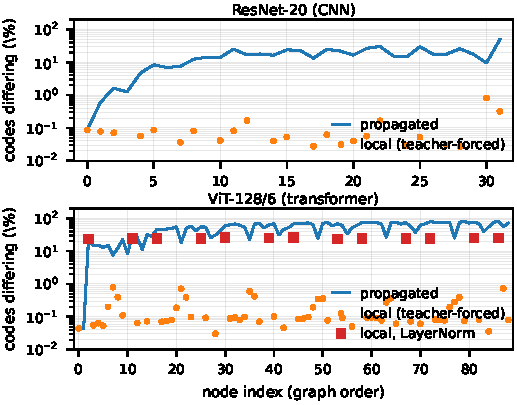
\includegraphics[width=\columnwidth]{fig1_decomposition.pdf}
\caption{Per-node code mismatch, \textsc{pc} scheme. Local (teacher-forced) mismatch is below $1\%$ for every operator except
LayerNorm; propagated mismatch rises from the first convolution to $50$--$73\%$ at the output. Log scale; nodes with zero local
mismatch (lookup-table activations, residual additions) are not drawn.}
\label{fig:decomposition}
\end{figure}

\subsection{Where the divergence is born}
Fig.~\ref{fig:decomposition} separates the two components. Local mismatch is small and flat: convolution disagrees on
$0.02$--$0.93\%$ of its codes, linear on $0.03$--$0.96\%$, average pooling on $0.1$--$2.7\%$ (rounding ties), and the int8
lookup-table activations on exactly $0\%$. Every one of these is a $\pm 1$ least-significant-bit disagreement. Propagated
mismatch, by contrast, rises monotonically from the first convolution --- the first divergence is that node in all twelve rows ---
and reaches $28$--$73\%$ at the output.

The transformer adds one operator that is not small: integer LayerNorm disagrees with its floating-point counterpart on
$24.8\%$ of its codes (maximum $26.2\%$ over the 13 instances). The integer implementation normalizes with an int64 sum and an
exact integer square root, while the simulator computes in float32 and then snaps to the grid, so roughly one element in four
lands on the other side of a rounding boundary. A practitioner porting a transformer to INT8 should suspect LayerNorm first.

\begin{table}[!t]
\caption{Making the simulator integer-faithful at LayerNorm (ViT-128/6, $10{,}000$ images). The integer program is unchanged
between the two rows of each scheme; only the simulator's LayerNorm differs. The mean absolute logit difference
falls from $0.119$ to $0.091$ (\textsc{pc}) and from $0.118$ to $0.093$ (\textsc{pt}).}
\label{tab:layernorm}
\centering
\footnotesize
\setlength{\tabcolsep}{4pt}
\begin{tabular}{llcccc}
\toprule
Sch. & LayerNorm & local (\%) & codes (\%) & agree (\%) & $\Delta$ (pp) \\
\midrule
\textsc{pc} & float32 & 24.77 & 72.7 & 97.93 & $+0.10\pm0.13$ \\
\textsc{pc} & integer (13) & 0.00 & 65.7 & 98.29 & $+0.25\pm0.11$ \\
\textsc{pt} & float32 & 24.76 & 72.6 & 98.07 & $+0.20\pm0.12$ \\
\textsc{pt} & integer (13) & 0.00 & 66.0 & 98.60 & $+0.13\pm0.10$ \\
\bottomrule
\end{tabular}

\end{table}

\subsection{Removing the largest local source does not close the gap}
If the divergence were a sum of per-operator errors, removing the largest one would help proportionally. We test this directly:
the simulator's LayerNorm is replaced by a module that computes the engine's arithmetic on the input codes, bit-exact by
construction, while the exported integer program is unchanged (the experiment asserts this).

Table~\ref{tab:layernorm} shows the outcome. Local LayerNorm mismatch goes from $24.77\%$ to exactly $0.00\%$, and the mean
absolute logit difference improves by about $23\%$. The propagated output-code mismatch moves only from $72.7\%$ to $65.7\%$
(per-tensor: $72.6\% \rightarrow 66.0\%$). Removing the single largest local source --- an operator responsible for two orders of
magnitude more local disagreement than any other --- recovers about a tenth of the propagated gap, because what remains is the
amplification of $\pm 1$ LSB events from operators whose individual local mismatch is below $1\%$. Accuracy moves within about
two paired standard errors in either direction and cannot be read as an improvement.

The practical consequence is that bit-accurate verification vectors have to come from an integer implementation. Repairing a
floating-point simulator operator by operator converges too slowly to be a substitute.

\begin{figure}[!t]
\centering
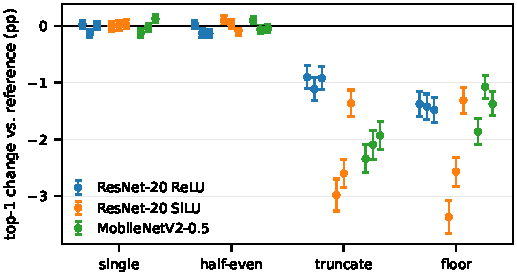
\includegraphics[width=\columnwidth]{fig2_rounding.pdf}
\caption{Top-1 change against the reference requantization rounding, complete test split, three independently trained
checkpoints per network (error bars: paired standard error). The biased modes lose in every combination; how much they lose
varies by seed.}
\label{fig:rounding}
\end{figure}

\begin{table}[!t]
\caption{Rounding-mode cost against the reference implementation, mean $\pm$ standard deviation over three seeds (pp).}
\label{tab:rounding}
\centering
\footnotesize
\input{tab3_rows}
\end{table}

\subsection{A cost the accuracy proxy hides}
The requantization multiply-and-shift ends in a rounding step, and an implementation may be tempted to replace it with a plain
arithmetic shift. Fig.~\ref{fig:rounding} and Table~\ref{tab:rounding} measure that choice against the reference implementation
on full test splits, with three independently trained checkpoints per network.

Two results. First, the \emph{sign and significance} are seed-robust: \texttt{truncate} and \texttt{floor} are worse than the
reference in all 18 (model, seed, mode) combinations, by $0.90$--$3.37$~pp, with $|\Delta|/\mathrm{SE}$ between $4.4$ and
$11.8$; the alternative single-rounding and round-half-to-even paths stay within noise ($|\Delta| \leq 0.13$~pp). Second, the
\emph{magnitude} is not: for ResNet-20 SiLU the cost of \texttt{truncate} ranges from $1.36$ to $2.98$~pp across three seeds, a
seed standard deviation equal to $37\%$ of the effect, while ResNet-20 ReLU stays within a tenth of its effect. Which of the two
biased modes is worse is a property of the network, not of the arithmetic: \texttt{floor} loses more on all three ResNet-20 ReLU
seeds, \texttt{truncate} loses more on all three MobileNetV2 seeds. A single-seed number should not be quoted as the cost of a
rounding mode.

\section{Related Work}
MQBench~\cite{mqbench} measures the gap between academic quantization and deployable backends, reporting it as accuracy;
the quantization white papers~\cite{nagel2021,krishnamoorthi2018} treat fake quantization as the simulation of the integer
pipeline. Layer-wise error analyses in deployment toolchains quantify how far a quantized layer is from its \emph{float}
counterpart. The measurement here is different in kind: how far the \emph{simulator} is from the \emph{integer execution} that
the device performs, in codes rather than in signal-to-noise ratio. Integer-only transformer inference has established integer
LayerNorm and softmax kernels~\cite{ibert,fqvit}; our contribution on that operator is not the kernel but the quantification of
its disagreement with the simulator, and the demonstration that fixing it is not sufficient. Accumulator width has been studied
as a training-time constraint~\cite{a2q}; the axis measured here is instead the rounding of the requantization step, which is a
pure implementation choice.

\section{Limitations}
The networks are CIFAR-10 scale plus one Imagenette model at $128\times128$; the conclusions are about the structure of the
divergence rather than its exact size on ImageNet-scale graphs. Three seeds cover the rounding axis only; the remaining
measurements use one checkpoint per network. The twelve accuracy comparisons in Table~\ref{tab:fidelity} and the four in
Table~\ref{tab:layernorm} are not corrected for multiple comparisons (over all sixteen, the largest $|\Delta|/\mathrm{SE}$ is
$2.2$). The external bit-exactness check covers convolution, pooling and fully-connected layers; depthwise convolution,
element-wise addition and softmax are not covered by it.

\section{Reproducibility}
Every number in this letter is emitted by a script from a committed result file, and the scripts, the trained checkpoints and
those result files are public. \texttt{python paper/make\_tables.py} regenerates Tables~\ref{tab:fidelity}--\ref{tab:rounding}
and \texttt{python paper/make\_figs.py} regenerates Figs.~\ref{fig:decomposition}--\ref{fig:rounding}; a continuous-integration
job re-runs the generators on every commit and fails if a committed table differs from the one the results imply. The
measurements themselves are \texttt{experiments/e15\_fidelity.py} (Table~\ref{tab:fidelity} and Fig.~\ref{fig:decomposition}),
\texttt{e16\_ln\_emulation.py} (Table~\ref{tab:layernorm}) and \texttt{e14\_rounding\_seeds.py}
(Fig.~\ref{fig:rounding}, Table~\ref{tab:rounding}); the external bit-exactness check is \texttt{e11\_tflite\_crosscheck.py}.
One caveat applies to the seeded measurement: the trainer's seed controlled data order but not weight initialization when these
checkpoints were produced, so the three replicates are independent draws that the same command will not reproduce bit for bit.

\section{Conclusion}
Simulated quantization predicts INT8 accuracy well and predicts INT8 tensors badly, and the two facts are independent. The gap
is not carried by any single operator: it is born as $\pm 1$ LSB events in operators that individually disagree on less than
$1\%$ of their codes, and it is grown by propagation, which is why removing the worst local source recovers only a tenth of it.
Teams that need golden vectors should generate them from an integer implementation validated against an external reference, and
teams that change a requantization detail should measure it across seeds, because its magnitude --- unlike its sign --- does not
transfer.

\section*{Acknowledgment}
% IEEE requires disclosure of AI-assisted content. Edit to match what you actually used before submitting.
The author used an AI assistant (Claude Code) for parts of the implementation, the experiment scripts and the drafting of this
manuscript. All experiments were executed by the author, and all reported numbers are produced by committed scripts from
committed result files.

% balance the final page: references 5-8 start the right column
\IEEEtriggeratref{5}
\begin{thebibliography}{10}
\bibitem{jacob2018} B.~Jacob \emph{et al.}, ``Quantization and training of neural networks for efficient integer-arithmetic-only
inference,'' in \emph{Proc. IEEE/CVF Conf. Comput. Vis. Pattern Recognit. (CVPR)}, 2018, pp. 2704--2713.
\bibitem{krishnamoorthi2018} R.~Krishnamoorthi, ``Quantizing deep convolutional networks for efficient inference: A whitepaper,''
\emph{arXiv:1806.08342}, 2018.
\bibitem{gemmlowp} B.~Jacob \emph{et al.}, ``gemmlowp: a small self-contained low-precision GEMM library,'' 2017. [Online].
Available: \url{https://github.com/google/gemmlowp}
\bibitem{nagel2021} M.~Nagel \emph{et al.}, ``A white paper on neural network quantization,'' \emph{arXiv:2106.08295}, 2021.
\bibitem{mqbench} Y.~Li \emph{et al.}, ``MQBench: Towards reproducible and deployable model quantization benchmark,'' in
\emph{Proc. NeurIPS Datasets and Benchmarks Track}, 2021.
\bibitem{ibert} S.~Kim \emph{et al.}, ``I-BERT: Integer-only BERT quantization,'' in \emph{Proc. Int. Conf. Mach. Learn. (ICML)},
2021, pp. 5506--5518.
\bibitem{fqvit} Y.~Lin \emph{et al.}, ``FQ-ViT: Post-training quantization for fully quantized vision transformer,'' in
\emph{Proc. Int. Joint Conf. Artif. Intell. (IJCAI)}, 2022, pp. 1173--1179.
\bibitem{a2q} I.~Colbert \emph{et al.}, ``A2Q: Accumulator-aware quantization with guaranteed overflow avoidance,'' in
\emph{Proc. IEEE/CVF Int. Conf. Comput. Vis. (ICCV)}, 2023, pp. 16989--16998.
\end{thebibliography}

\end{document}
